
\section{Classification}

In this section, we will be covering the basics of classification machine learning techniques. Topics
will range from what data to use for learning, how to train a Multiclass/binary classifiers, 
look over different performance measures and finally looking over multioutput classifiers. 

\subsection{MNIST}

In this section we will be utilizing the MNIST dataset, which is made up of 70,000 images of digits
written by hand. Each image is labeled with the digit it is an image of. This is one of the most 
popular datasets for intially learning about the world of Machine Learning (Equivalent to the 
"Hello World" program when first learning how to code).\\

\noindent
Fortunately, Scikit-Learn provides a very easy way to obtain this data. Using the following block
of code we can obtain this dataset:

\begin{minted}{python}
from sklearn.datasets import fetch_openml
mnist = fetch_openml("mnist_784", version=1)
mnist.keys()

# Below will be the dictionary for this dataset
'''
dict_keys(['data', 'target', 'feature_names', 'DESCR', 'details',
           'categories', 'url'])
'''
\end{minted}

\noindent
Datasets from Scikit-Learn have mostly the same dictionary structure:

\begin{itemize}
    \item A \mintinline{python}{DESCR} key describes the dataset
    \item A \mintinline{python}{data} key contains an array with one row per instance and one column
    per feature
    \item A \mintinline{python}{target} key containing an array with all the labels for each respective
    image that is in the data
\end{itemize}

\noindent
Lets take a look at the shape of the dataset:

\begin{minted}{python}
X, y = mnist["data"], mnist["target"]
X.shape # (70000, 784)
y.shape # (70000,)    
\end{minted}

\noindent 
Here we see, as mentioned earlier, that there is 70,000 images with each image containing 784 
features. There are 784 features as each image is 28 x 28 pixels, and each feature represents the pixels
density ranging from 0 (white) to 255 (black). Additionally, we see that the target data is just 
70,000 labels for each respective image in X. \\ 

\noindent
Finally, we should always split the data before inspecting the data more closely. We can make the 
test and training sets in the following manner:

\begin{minted}{python}
X_train, X_test = X[:60000], X[60000:]
y_train, y_test = y[:60000], y[60000:]    
\end{minted}

\noindent
\textbf{Note:} that this dataset has already been shuffled. However, if this dataset has not been
shuffled then it is crucial that we do this before splitting the data as we do not want some folds
when doing cross-validation to be missing digits.

\subsection{Training a Binary Classifier}

For simplification reasons, we will first only try to identify one digit, number 5. This classifier 
will be a \textit{binary classifier}, capable of distinguishing between just 2 classes 5 and not a 5.\\

\noindent
First we will create target vectors for this classification task:

\begin{minted}{python}
y_train_5 = (y_train == 5) # True for all 5s, False for all others
y_test_5 = (y_test == 5)
\end{minted}

For this example we will be using the \textit{Stochastic Gradient Descent} (SGD) classifier, using 
Scikit-Learn's \mintinline{python}{SGDClassifier} class. This classifier is advantageous because it 
is able to handle large datasets efficiently. This is the calse because SGD deals with training instances
independently, one at a time.\\

\noindent
Below will be some code that is implementing this classifier:

\begin{minted}{python}
from sklern.linear_model import SGDClassifier

sgd_clf = SGDClassifier(random_state=42)
sgd_clf.fit(X_train_5, y_test_5)    
\end{minted}

\noindent
Now that the model is trained we, hope, that we can now predict with reasonable accuracy that a 
number is a 5 and not a 5 if it is some other digit.

\subsection{Performance Measures}

Here we find that evaluating a classifier tends to be much trickier than evaluating a regression based
model. In this section, we will be spending a lot of time going over the many different performance
measures there are available. 

\subsubsection{Measuring Accuracy Using Cross-Validation}

A common way to evaluate a model is to just use cross-validation. Here we will be using a off the shelf
cross validation function, but if you need more control over the cross-validation processs then you 
can always build your own. \\

\noindent
Below will be the implementation using Sciki-Learn's \mintinline{python}{cross_val_score()} function
to evaluate our \mintinline{python}{SGDClassifier} we trained earlier. Note, that we are using K-folds
cross-validation when using the python function \mintinline{python}{cross_val_score()}.

\begin{minted}{python}
from sklearn.model_selection import cross_val_score
# Splits training set into 3 folds, then making predictions and 
# evaluating them on each fold using a model trained on the remaining
# folds.
cross_val_score(sgd_clf, X_train, y_train, cv = 3, scoring='accuracy')

# Output:
# array([0.96355, 0.93795, 0.95615])
\end{minted}

\noindent
After cross-validation we see that the model has an accuracy of above 93\% on all cross-validation 
folds. However, there is a catch to this. We will now fit a "very dumb" classifier that just 
classifies every image as a "not-5" class:

\begin{minted}{python}
from sklearn.base import BaseEstimator

class Never5Classifier(BaseEstimator):
    def fit(self, X, y=None):
        pass
    def predict(self, X):
        return np.zeros((len(x), 1), dtype=bool)

never_5_clf = Never5Classifier()
cross_val_score(never_5_clf, X_train, y_train, cv=3, scoring='accuracy')

# Output:
# array([0.91125, 0.90855, 0.90915])
\end{minted}

\noindent
Woah, we have over 90\% accuracy on the dataset by just classifying everything as not a 5. This is 
because we only have about 10\% of the images as 5s, so if we always guess that the image is not a 
5 then we will be right about 90\% of the time. \\

\noindent 
The above is a prime example why accuracy is generally not the preferred performance measure for 
classifiers, especially when we are dealing with \textit{skewed datasets} (i.e., when some classes
are much more frequent then others).

\subsubsection{Confusion Matrix}

Another way to evaluate performance of a classfier is to look at the \textit{Confusion Matrix}. In
general, the idea of this matrix is to count the number of times instances of a class A are classified
as a class B. \\ 

\noindent
To create the confusion matrix, we need to first have a set of predictions so that they can be compared
to the actual targets. As we generally do not want to touch the test set until the model is complete,
we can use \mintinline{python}{cross_val_predict()} instead to generate our predictions against the 
target:

\begin{minted}{python}
from sklearn.model_selection import cross_val_predict()
from sklearn.metrics import confusion_matrix

y_train_pred = cross_val_predict(sgd_clf, X_train, y_train_5, cv=3)

confusion_matrix(y_train_5, y_train_pred)

'''
Output:
Confusion Matrix Below:
array([[53057,  1522],
       [ 1325,  4096]])
'''
\end{minted}

\noindent
Similarly as above, \mintinline{python}{cross_val_predict()}, also performs K-fold cross-validation,
but instead of returning scores, it returns the predictions made on each test fold. Now for the
confusion matrix:\\

\noindent 
\textbf{Confusion Matrix Explanation}
\begin{itemize}
    \item Each \textbf{Row} in a confusion matrix represents an \textit{actual class}
    \item Each \textbf{Column} in a confusion matrix represents a \textit{predicted class}
\end{itemize}

\noindent
In the case for this model, the \textbf{first row} of the matrix above considers non-5 images (negative class):
53,057 of them were correctly classified as non-5s (called \textit{True Negatives}), while the 
remaining 1,522 were wrongly classified as 5s (\textit{False Positives}). The \textbf{second row}, 
considers the images of 5s (\textit{positive class}): 1,325 were wrongly classified as non-5s 
(\textit{false negatives}), while the remaining 4,096 were correctly classified as 5s (\textit{True Positives}).
Additionally, a perfect classifier would only have non-zero values on the main diagonal. 

\subsubsection{Precision and Recall}

Although the \textit{confusion matrix} may give a lot of information, sometimes it is better to look at a more 
straight-forward metric. Both \textit{Precision} and \textit{Recall} are great for this task.

\subsubsection*{Precision}

\textit{Precision}, can be defined as the accuracy of the positive prediction for the classifier we are evaluating.
Below will be the formula to calculate precision:

$$\text{Precision} = \frac{\text{TP}}{\text{TP} + \text{FP}}$$

\noindent 
Where:
\begin{itemize}
    \item TP $\rightarrow$ The number of true positives
    \item FP $\rightarrow$ The number of false positives
\end{itemize}

\subsubsection*{Recall}

\textit{Recall}, can be defined as the \textit{sensitivity} or the \textit{true positive rate} (TPR):
this is the ratio of positive instances that are correctly detected by the classifier. The 
equation for Recall can be defined as follows:

$$\text{Recall} = \frac{\text{TP}}{\text{TP} + \text{FN}}$$

\noindent
Where, FN, is the number of false negatives. Additionally, below we can see a more detailed 
version of the confusion matrix to help clear any confusion:

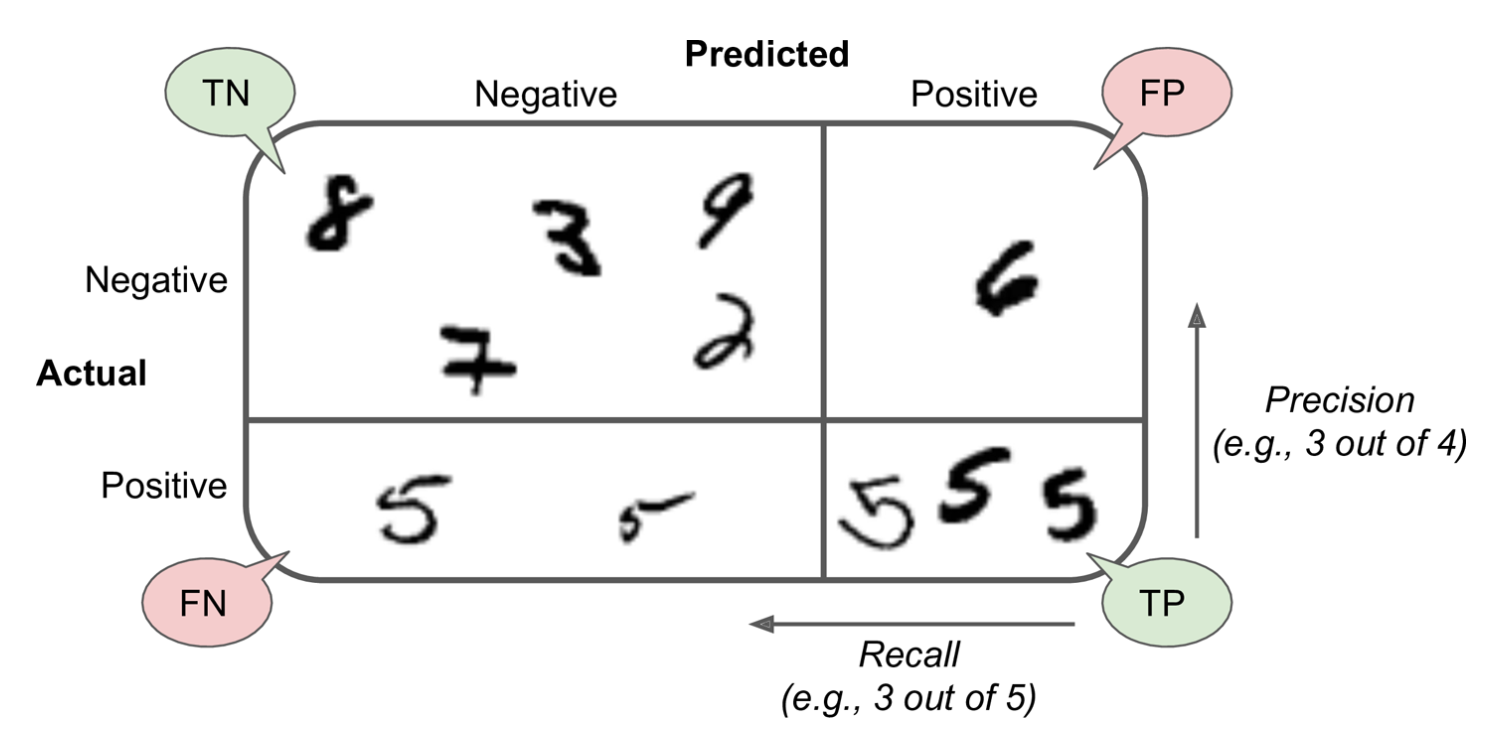
\includegraphics[scale=0.65]{Images/ConfusionMatrix.PNG}

\subsubsection*{Precision and Recall}

Scikit-Learn provides several functions to help compute classifier metrics, including precision
and recall. See below an example:

\pagebreak

\begin{minted}{python}
from sklearn.metrics import precision_score, recall_score

precision_score(y_train_5, y_train_pred) # == 4096 / (4096 + 1522)
# Output: 0.7291

recall_score(y_train_5, y_train_pred) # == 4096 / (4096 + 1325)
# Output: 0.7556
\end{minted}

\noindent
Now we can see that the classifier is definitely not as good as we originally thought. From 
\textbf{Precision}, we now see that when the classifier claims an image is of a 5, it is only 
correct about 72.9\% of the time. Additionally, from \textbf{Recall}, we can see that the classifier 
only detects 75.6\% of the 5s. \\

\noindent
In addition, we often find it useful to combine both precision and recall into a single metric which is 
known as the $\mathbf{F_{1} \textbf{ score}}$. This new metric can be defined as follows:

$$\mathbf{F_{1}} = \frac{2}{\frac{1}{\text{precision}} + \frac{1}{\text{recall}}} = 2 \times \frac{\text{Precision} \times \text{Recall}}{{\text{Precision}} + \text{Recall}} = \frac{\text{TP}}{\text{TP} + \frac{\text{FN} + \text{FP}}{2}}$$

\noindent
As follows, Scikit-Learn has a built in function for this as well. We can call \mintinline{python}{f1_score()}
function.

\begin{minted}{python}
from sklearn.metrics import f1_score
f1_score(y_train_5, y_train_pred)
# Output: 0.7421    
\end{minted}

\noindent
\textbf{Note}: that the $F_{1}$ score favors classifiers that have similar precision and recall. This may not 
always be that case that we want. Some cases may call for mostly caring about precision, and on other cases it 
may be best to only care a lot about recall. \\

\noindent
We can also not have both high precision and recall, as if we increase one the other tends to decrease. This is known
as the \textit{Precision/Recall Trade-Off}.

\subsubsection{ROC Curve}

The \textit{Revceiver Operating Characteristic} (ROC) curve is another common way to evaluate a binary classifiers
ability to predict correct classes. The ROC curve is created by plotting the \textit{True Positive Rate} (Also 
known as Recall) against the \textit{False Positive Rate} (FPR). The FPR is the ratio of negative instances that are
incorrectly classified as positive. It is also equal to $1 -$ the \textit{True Negative Rate} (TNR), which is the 
ratio of negative instances that are correctly classified as negative. TNR is also called \textit{Specificity}. \\

\noindent 
\textbf{Note}: As a general rule, it is better to use the \textit{Precision/Recall Curve} when the positive class is
rare or when we care more about the false positive than the false negatives. Otherwise, it is better to use the ROC
curve. 

\subsection{Multiclass Classifification}

In this section we will be discussing how we can train classifiers that are choosing between more than just 
two separate classes. Some algorithms (SGD classifiers, Random Forest Classifiers, and Naive Bayes Classifiers) are 
capable of handling multiple classes natively. However, others (Logisitc Regression, SVM) are strictly binary
classifiers, but as we will see, there are strategies so that we can perform multiclass classification with 
binary classifiers. \\

\noindent
There are 2 strategies for making it possible for binary classifiers to have the ability to classify multiple 
classes. The strategies are known as \textbf{One-Versus-Rest} (OvR) and \textbf{One-Versus-One} (OvO).

\subsubsection*{One-Versus-Rest}

This strategy is fairly basic in that, for example, if we want to train binary classifiers to classify digit images
into 10 classes (0 to 9), we can train 10 binary classifiers, one for each digit (0-detector, 1-detector, etc.). Then
when we want to classify an image, we get a decision score from each classifier for that image and we select the 
class whose classifier outputs the highest score.

\subsubsection*{One-Versus-One}

The second strategy is to train binary classifiers for every pair of digits to distinguish 0s and 1s, 0s and 2s, 
1s and 2s, and so on. If there are N classes then we will need to train $\frac{N(N-1)}{2}$ classifiers. For the 
MNIST data we will need to train 45 binary classifiers. When we want to classify an image, we have to run the image
through all 45 classifiers and see which class wins the most duels. The main advantage of this strategy is that each
classifier only needs to be trained on a part of the training set for the two classes it must distinguish. \\

\noindent
However, some algorithms, such as SVM, scale very poorly with size of the training set. Therefore, it is preferred that
these algorithm use the OvO strategy as it is faster to train several classifiers on small training sets than a few
on large training sets (Although in most cases for binary classifiers, OvR is preferred).
